\documentclass[10pt,a4paper]{article}
\usepackage[margin=0.5in]{geometry}
\usepackage{amsmath,amssymb}
\usepackage{tikz}
\usetikzlibrary{shapes.geometric,arrows.meta,positioning,calc,fit,backgrounds}
\usepackage{times}

\pagestyle{empty}

\begin{document}

\begin{center}
{\LARGE \textbf{Figure 4.1: Framework of PrismSpace Multi-Agent System}}\\[1.2em]

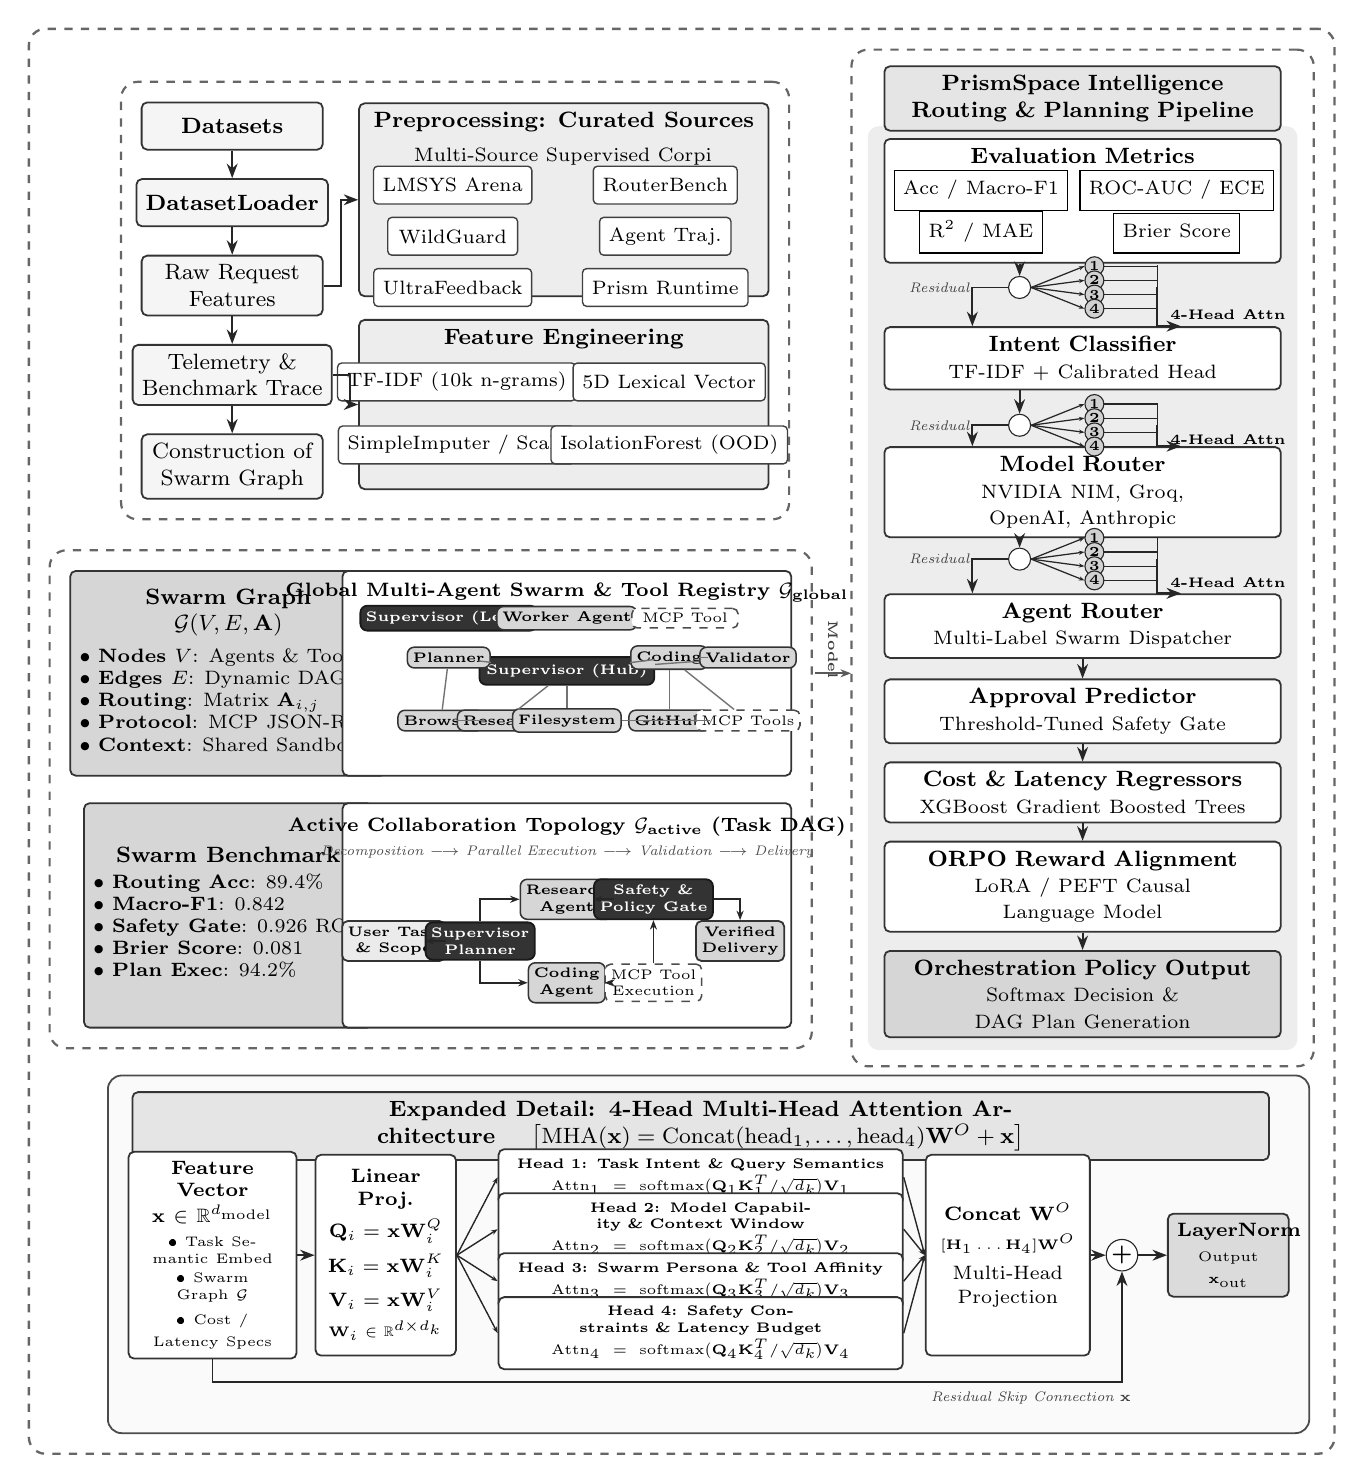
\begin{tikzpicture}[
    auto,
    font=\footnotesize,
    box/.style = {
        rectangle,
        draw=black!80,
        line width=0.65pt,
        fill=black!4,
        rounded corners=2pt,
        align=center
    },
    mini_box/.style = {
        rectangle,
        draw=black!75,
        line width=0.5pt,
        fill=white,
        rounded corners=1.5pt,
        minimum height=0.48cm,
        minimum width=1.65cm,
        align=center,
        font=\scriptsize
    },
    shaded_col/.style = {
        rectangle,
        draw=black!80,
        line width=0.65pt,
        fill=black!16,
        rounded corners=2pt,
        align=center
    },
    arrow/.style = {
        -{Stealth[scale=0.85]},
        line width=0.7pt,
        draw=black!85
    },
    dashed_container/.style = {
        draw=black!60,
        dashed,
        line width=0.8pt,
        rounded corners=6pt
    },
    head_box/.style = {
        rectangle,
        draw=black!75,
        line width=0.5pt,
        fill=black!5,
        rounded corners=2pt,
        minimum height=0.38cm,
        minimum width=5.6cm,
        font=\fontsize{4.8}{5.8}\selectfont,
        align=center
    },
    agent_node/.style = {
        circle,
        draw=black!85,
        line width=0.7pt,
        fill=black!30,
        inner sep=0pt,
        minimum size=0.42cm
    },
    eval_node/.style = {
        circle,
        draw=black!85,
        line width=0.7pt,
        fill=black!75,
        inner sep=0pt,
        minimum size=0.42cm
    }
]

    % =========================================================================
    % TOP-LEFT PANEL: DATASET INGESTION & PREPROCESSING
    % =========================================================================
    
    % Left-side vertical pipeline in Top-Left
    \node [box, minimum width=2.3cm, minimum height=0.6cm] (ds) at (-4.5, 5.2) {\textbf{Datasets}};
    \node [box, minimum width=2.3cm, minimum height=0.6cm, below=0.35cm of ds] (loader) {\textbf{DatasetLoader}};
    \node [box, minimum width=2.3cm, minimum height=0.65cm, below=0.35cm of loader] (raw_feat) {Raw Request\\Features};
    \node [box, minimum width=2.3cm, minimum height=0.65cm, below=0.35cm of raw_feat] (pop_feat) {Telemetry \&\\Benchmark Trace};
    \node [box, minimum width=2.3cm, minimum height=0.65cm, below=0.35cm of pop_feat] (sim_const) {Construction of\\Swarm Graph};

    \draw [arrow] (ds) -- (loader);
    \draw [arrow] (loader) -- (raw_feat);
    \draw [arrow] (raw_feat) -- (pop_feat);
    \draw [arrow] (pop_feat) -- (sim_const);

    % Right-side boxes in Top-Left: Curated Sources
    \node [box, fill=black!7, minimum width=5.2cm, minimum height=2.45cm, anchor=north west] (prep_box) at (-2.9, 5.5) {};
    \node [anchor=north, font=\footnotesize\bfseries] at (prep_box.north) {Preprocessing: Curated Sources};
    \node [font=\scriptsize, anchor=north] at (-0.3, 5.05) {Multi-Source Supervised Corpi};

    % 6 mini boxes inside Curated Sources
    \node [mini_box] (mb1) at (-1.7, 4.45) {LMSYS Arena};
    \node [mini_box] (mb2) at (1.0, 4.45) {RouterBench};
    \node [mini_box] (mb3) at (-1.7, 3.8) {WildGuard};
    \node [mini_box] (mb4) at (1.0, 3.8) {Agent Traj.};
    \node [mini_box] (mb5) at (-1.7, 3.15) {UltraFeedback};
    \node [mini_box] (mb6) at (1.0, 3.15) {Prism Runtime};

    % Preprocessed Features Box
    \node [box, fill=black!7, minimum width=5.2cm, minimum height=2.15cm, anchor=north west] (feat_box) at (-2.9, 2.75) {};
    \node [anchor=north, font=\footnotesize\bfseries] at (feat_box.north) {Feature Engineering};
    \node [mini_box, minimum width=2.2cm] (tf1) at (-1.65, 1.95) {TF-IDF (10k n-grams)};
    \node [mini_box, minimum width=2.2cm] (tf2) at (1.05, 1.95) {5D Lexical Vector};
    \node [mini_box, minimum width=2.2cm] (tf3) at (-1.65, 1.15) {SimpleImputer / Scale};
    \node [mini_box, minimum width=2.2cm] (tf4) at (1.05, 1.15) {IsolationForest (OOD)};

    % Stepped arrows from left ingestion pipeline into preprocessing & feature engineering
    \draw [arrow] (raw_feat.east) -- ++(0.22, 0) |- (prep_box.west);
    \draw [arrow] (pop_feat.east) -- ++(0.22, 0) |- (feat_box.west);

    % Top-left container boundary
    \node [dashed_container, fit=(ds) (sim_const) (prep_box) (feat_box), inner sep=0.25cm] (container_topleft) {};

    % Node styles for expanded Swarm Graph
    \tikzset{
        swarm_node/.style = {
            rounded corners=2.5pt,
            draw=black!80,
            line width=0.55pt,
            fill=black!16,
            font=\fontsize{5}{6}\selectfont\bfseries,
            inner sep=2pt,
            align=center
        },
        super_node/.style = {
            rounded corners=2.5pt,
            draw=black!90,
            line width=0.65pt,
            fill=black!80,
            text=white,
            font=\fontsize{5}{6}\selectfont\bfseries,
            inner sep=2pt,
            align=center
        },
        tool_node/.style = {
            rounded corners=2pt,
            draw=black!70,
            dashed,
            line width=0.55pt,
            fill=white,
            font=\fontsize{5}{6}\selectfont,
            inner sep=1.8pt,
            align=center
        }
    }

    % =========================================================================
    % BOTTOM-LEFT PANEL: AGENT SWARM GRAPH & EVALUATION (EXPANDED)
    % =========================================================================
    
    \node [shaded_col, minimum width=2.45cm, minimum height=2.6cm] (sim_graph_lbl) at (-4.55, -1.75) {
        \textbf{Swarm Graph}\\
        $\mathcal{G}(V, E, \mathbf{A})$\\[0.35em]
        \scriptsize
        \begin{tabular}{@{}l@{}}
        $\bullet$ \textbf{Nodes $V$}: Agents \& Tools\\
        $\bullet$ \textbf{Edges $E$}: Dynamic DAG\\
        $\bullet$ \textbf{Routing}: Matrix $\mathbf{A}_{i,j}$\\
        $\bullet$ \textbf{Protocol}: MCP JSON-RPC\\
        $\bullet$ \textbf{Context}: Shared Sandbox
        \end{tabular}
    };

    \node [shaded_col, minimum width=2.45cm, minimum height=2.85cm] (eval_lbl) at (-4.55, -4.825) {
        \textbf{Swarm Benchmark}\\[0.3em]
        \scriptsize
        \begin{tabular}{@{}l@{}}
        $\bullet$ \textbf{Routing Acc}: 89.4\%\\
        $\bullet$ \textbf{Macro-F1}: 0.842\\
        $\bullet$ \textbf{Safety Gate}: 0.926 ROC\\
        $\bullet$ \textbf{Brier Score}: 0.081\\
        $\bullet$ \textbf{Plan Exec}: 94.2\%
        \end{tabular}
    };

    % Top Graph visual area: Global Swarm Mesh
    \node [box, fill=white, minimum width=5.7cm, minimum height=2.6cm] (graph_box_top) at (-0.25, -1.75) {};
    
    % Header & Legend
    \node [font=\scriptsize\bfseries] at (-0.25, -0.72) {Global Multi-Agent Swarm \& Tool Registry $\mathcal{G}_{\text{global}}$};
    \node [super_node, minimum width=1.45cm, font=\tiny\bfseries] at (-1.75, -1.05) {Supervisor (Lead)};
    \node [swarm_node, minimum width=1.35cm, font=\tiny\bfseries] at (-0.25, -1.05) {Worker Agent};
    \node [tool_node, minimum width=1.35cm, font=\tiny] at (1.25, -1.05) {MCP Tool};

    % Top Swarm Topological Nodes (Strictly non-overlapping positions)
    \node [super_node, font=\tiny\bfseries, inner sep=2.5pt] (s_super) at (-0.25, -1.72) {Supervisor (Hub)};
    \node [swarm_node, font=\tiny\bfseries, inner sep=2pt] (w_plan)  at (-1.75, -1.55) {Planner};
    \node [swarm_node, font=\tiny\bfseries, inner sep=2pt] (w_brow)  at (-1.85, -2.35) {Browser};
    \node [swarm_node, font=\tiny\bfseries, inner sep=2pt] (w_res)   at (-1.05, -2.35) {Research};
    \node [swarm_node, font=\tiny\bfseries, inner sep=2pt] (w_fs)    at (-0.25, -2.35) {Filesystem};
    \node [swarm_node, font=\tiny\bfseries, inner sep=2pt] (w_code)  at (1.05, -1.55)  {Coding};
    \node [swarm_node, font=\tiny\bfseries, inner sep=2pt] (w_git)   at (1.05, -2.35)  {GitHub};
    \node [swarm_node, font=\tiny\bfseries, inner sep=2pt] (w_val)   at (2.05, -1.55)  {Validator};
    \node [tool_node, font=\tiny, inner sep=2pt]  (t_mcp)   at (2.05, -2.35)  {MCP Tools};

    % Mesh Interconnections
    \draw [draw=black!55, line width=0.5pt] (s_super) -- (w_plan);
    \draw [draw=black!55, line width=0.5pt] (s_super) -- (w_code);
    \draw [draw=black!55, line width=0.5pt] (s_super) -- (w_res);
    \draw [draw=black!55, line width=0.5pt] (s_super) -- (w_fs);
    \draw [draw=black!55, line width=0.5pt] (s_super) -- (w_val);
    \draw [draw=black!55, line width=0.5pt] (w_plan) -- (w_brow);
    \draw [draw=black!55, line width=0.5pt] (w_brow) -- (w_res);
    \draw [draw=black!55, line width=0.5pt] (w_code) -- (w_git);
    \draw [draw=black!55, line width=0.5pt] (w_code) -- (w_val);
    \draw [draw=black!55, line width=0.5pt] (w_code) -- (t_mcp);
    \draw [draw=black!55, line width=0.5pt] (w_git) -- (t_mcp);
    \draw [draw=black!55, line width=0.5pt] (w_fs) -- (t_mcp);

    % Bottom Graph visual area: Active Collaboration DAG (EXPANDED)
    \node [box, fill=white, minimum width=5.7cm, minimum height=2.85cm] (graph_box_bot) at (-0.25, -4.825) {};
    \node [font=\scriptsize\bfseries] at (-0.25, -3.7) {Active Collaboration Topology $\mathcal{G}_{\text{active}}$ (Task DAG)};
    \node [font=\fontsize{4.8}{5.8}\selectfont\itshape, text=black!70] at (-0.25, -4.02) {Decomposition $\longrightarrow$ Parallel Execution $\longrightarrow$ Validation $\longrightarrow$ Delivery};

    % Active DAG Workflow Nodes (Symmetrically spaced, clean vertical layers, zero overlaps)
    \node [box, fill=black!8, font=\tiny\bfseries, inner sep=2pt, minimum width=0.88cm] (d_req) at (-2.45, -5.15) {User Task\\\& Scope};
    \node [super_node, font=\tiny\bfseries, inner sep=2pt, minimum width=0.88cm] (d_lead) at (-1.35, -5.15) {Supervisor\\Planner};
    \node [swarm_node, font=\tiny\bfseries, inner sep=2pt, minimum width=0.88cm] (d_res)  at (-0.25, -4.62) {Research\\Agent};
    \node [swarm_node, font=\tiny\bfseries, inner sep=2pt, minimum width=0.88cm] (d_code) at (-0.25, -5.68) {Coding\\Agent};
    \node [super_node, font=\tiny\bfseries, inner sep=2pt, minimum width=0.88cm] (d_gate) at (0.85, -4.62) {Safety \&\\Policy Gate};
    \node [tool_node, font=\tiny, inner sep=2pt, minimum width=0.88cm] (d_tool) at (0.85, -5.68) {MCP Tool\\Execution};
    \node [box, fill=black!16, font=\tiny\bfseries, inner sep=2pt, minimum width=0.88cm] (d_out) at (1.95, -5.15) {Verified\\Delivery};

    % Active Directed Workflow Connections
    \draw [-{Stealth[scale=0.6]}, line width=0.6pt, black!85] (d_req) -- (d_lead);
    \draw [-{Stealth[scale=0.6]}, line width=0.6pt, black!85] (d_lead) |- (d_res);
    \draw [-{Stealth[scale=0.6]}, line width=0.6pt, black!85] (d_lead) |- (d_code);
    \draw [{Stealth[scale=0.55]}-{Stealth[scale=0.55]}, line width=0.6pt, black!85] (d_code) -- (d_tool);
    \draw [-{Stealth[scale=0.6]}, line width=0.6pt, black!85] (d_res) -- (d_gate);
    \draw [-{Stealth[scale=0.6]}, line width=0.6pt, black!85] (d_tool) -- (d_gate);
    \draw [-{Stealth[scale=0.6]}, line width=0.6pt, black!85] (d_gate) -| (d_out);

    % Bottom-left container boundary
    \node [dashed_container, fit=(sim_graph_lbl) (eval_lbl) (graph_box_top) (graph_box_bot), inner sep=0.25cm] (container_botleft) {};

    % =========================================================================
    % RIGHT PANEL: ML ROUTING & PLANNING PIPELINE
    % =========================================================================
    
    \node [box, fill=black!10, text width=4.8cm, minimum height=0.68cm] (hdr_right) at (6.3, 5.55) {
        \textbf{PrismSpace Intelligence}\\
        \textbf{Routing \& Planning Pipeline}
    };

    \node [box, fill=white, text width=4.8cm, minimum height=0.82cm] (eval_box) at (6.3, 4.25) {
        \textbf{Evaluation Metrics}\\[0.15em]
        {\scriptsize
        \begin{tabular}{@{}c@{\hspace{0.5em}}c@{}}
        \fbox{\strut Acc / Macro-F1} & \fbox{\strut ROC-AUC / ECE} \\
        \fbox{\strut R$^2$ / MAE} & \fbox{\strut Brier Score}
        \end{tabular}}
    };

    % Stack of Layers matching Figure 4.1 structure with compact 4-Head Attention junctions
    % --- JUNCTION 1: Between Evaluation Metrics and Intent Classifier ---
    \node [circle, draw=black!85, fill=white, inner sep=0pt, minimum size=0.28cm] (circ1) at (5.5, 3.15) {};
    
    % Layer 1: Intent Classifier
    \node [box, fill=white, text width=4.8cm, minimum height=0.56cm] (l1) at (6.3, 2.25) {
        \textbf{Intent Classifier}\\
        \scriptsize TF-IDF + Calibrated Head
    };

    % --- JUNCTION 2: Between Intent Classifier and Model Router ---
    \node [circle, draw=black!85, fill=white, inner sep=0pt, minimum size=0.28cm] (circ2) at (5.5, 1.40) {};
    
    % Layer 2: Model Router
    \node [box, fill=white, text width=4.8cm, minimum height=0.56cm] (l2) at (6.3, 0.55) {
        \textbf{Model Router}\\
        \scriptsize NVIDIA NIM, Groq, OpenAI, Anthropic
    };

    % --- JUNCTION 3: Between Model Router and Agent Router ---
    \node [circle, draw=black!85, fill=white, inner sep=0pt, minimum size=0.28cm] (circ3) at (5.5, -0.30) {};
    
    % Layer 3: Agent Router
    \node [box, fill=white, text width=4.8cm, minimum height=0.56cm] (l3) at (6.3, -1.15) {
        \textbf{Agent Router}\\
        \scriptsize Multi-Label Swarm Dispatcher
    };

    \node [box, fill=white, text width=4.8cm, minimum height=0.56cm, below=0.25cm of l3] (l4) {
        \textbf{Approval Predictor}\\
        \scriptsize Threshold-Tuned Safety Gate
    };

    \node [box, fill=white, text width=4.8cm, minimum height=0.56cm, below=0.22cm of l4] (jk) {
        \textbf{Cost \& Latency Regressors}\\
        \scriptsize XGBoost Gradient Boosted Trees
    };

    \node [box, fill=white, text width=4.8cm, minimum height=0.56cm, below=0.22cm of jk] (fc) {
        \textbf{ORPO Reward Alignment}\\
        \scriptsize LoRA / PEFT Causal Language Model
    };

    \node [box, fill=black!16, text width=4.8cm, minimum height=0.56cm, below=0.22cm of fc] (sig) {
        \textbf{Orchestration Policy Output}\\
        \scriptsize Softmax Decision \& DAG Plan Generation
    };

    % Behind-the-stack vertical shaded backing (matching Figure 4.1 in paper)
    \begin{scope}[on background layer]
        \node [draw=none, fill=black!7, rounded corners=4pt, fit=(eval_box) (sig), inner xsep=0.2cm, inner ysep=0.15cm] (bg_stack) {};
    \end{scope}

    % --- ARROW FLOW IN COMPACT RIGHT PIPELINE ---
    
    % --- JUNCTION 1 DETAILS ---
    \draw [arrow] (eval_box.south -| circ1) -- (circ1);
    
    % Residual / Skip Branch
    \draw [arrow] (circ1.west) -| node[pos=0.4, left, font=\fontsize{4.5}{5.5}\selectfont\itshape, text=black!75]{Residual} ($(l1.north)+(-1.4, 0)$);

    % Compact 4-Head Attention Fan-out
    \node [circle, draw=black!85, fill=black!18, inner sep=0pt, minimum size=0.24cm, font=\fontsize{4.2}{5.2}\selectfont\bfseries] (h1_1) at (6.45, 3.42) {1};
    \node [circle, draw=black!85, fill=black!18, inner sep=0pt, minimum size=0.24cm, font=\fontsize{4.2}{5.2}\selectfont\bfseries] (h1_2) at (6.45, 3.24) {2};
    \node [circle, draw=black!85, fill=black!18, inner sep=0pt, minimum size=0.24cm, font=\fontsize{4.2}{5.2}\selectfont\bfseries] (h1_3) at (6.45, 3.06) {3};
    \node [circle, draw=black!85, fill=black!18, inner sep=0pt, minimum size=0.24cm, font=\fontsize{4.2}{5.2}\selectfont\bfseries] (h1_4) at (6.45, 2.88) {4};

    \draw [-{Stealth[scale=0.4]}, line width=0.45pt, black!85] (circ1.east) -- (h1_1.west);
    \draw [-{Stealth[scale=0.4]}, line width=0.45pt, black!85] (circ1.east) -- (h1_2.west);
    \draw [-{Stealth[scale=0.4]}, line width=0.45pt, black!85] (circ1.east) -- (h1_3.west);
    \draw [-{Stealth[scale=0.4]}, line width=0.45pt, black!85] (circ1.east) -- (h1_4.west);

    \coordinate (m_conv1) at (7.25, 3.15);
    \draw [line width=0.45pt, black!85] (h1_1.east) -- (h1_1.east -| m_conv1);
    \draw [line width=0.45pt, black!85] (h1_2.east) -- (h1_2.east -| m_conv1);
    \draw [line width=0.45pt, black!85] (h1_3.east) -- (h1_3.east -| m_conv1);
    \draw [line width=0.45pt, black!85] (h1_4.east) -- (h1_4.east -| m_conv1);
    \draw [line width=0.6pt, black!85] ($(m_conv1)+(0, 0.28)$) -- ($(m_conv1)+(0, -0.28)$);
    \draw [arrow] (m_conv1) |- node[pos=0.35, right, font=\fontsize{4.8}{5.8}\selectfont\bfseries, xshift=1pt]{4-Head Attn} ($(l1.north)+(1.25, 0)$);

    % --- JUNCTION 2 DETAILS ---
    \draw [arrow] (l1.south -| circ2) -- (circ2);
    
    % Residual / Skip Branch
    \draw [arrow] (circ2.west) -| node[pos=0.4, left, font=\fontsize{4.5}{5.5}\selectfont\itshape, text=black!75]{Residual} ($(l2.north)+(-1.4, 0)$);

    % Compact 4-Head Attention Fan-out
    \node [circle, draw=black!85, fill=black!18, inner sep=0pt, minimum size=0.24cm, font=\fontsize{4.2}{5.2}\selectfont\bfseries] (h2_1) at (6.45, 1.67) {1};
    \node [circle, draw=black!85, fill=black!18, inner sep=0pt, minimum size=0.24cm, font=\fontsize{4.2}{5.2}\selectfont\bfseries] (h2_2) at (6.45, 1.49) {2};
    \node [circle, draw=black!85, fill=black!18, inner sep=0pt, minimum size=0.24cm, font=\fontsize{4.2}{5.2}\selectfont\bfseries] (h2_3) at (6.45, 1.31) {3};
    \node [circle, draw=black!85, fill=black!18, inner sep=0pt, minimum size=0.24cm, font=\fontsize{4.2}{5.2}\selectfont\bfseries] (h2_4) at (6.45, 1.13) {4};

    \draw [-{Stealth[scale=0.4]}, line width=0.45pt, black!85] (circ2.east) -- (h2_1.west);
    \draw [-{Stealth[scale=0.4]}, line width=0.45pt, black!85] (circ2.east) -- (h2_2.west);
    \draw [-{Stealth[scale=0.4]}, line width=0.45pt, black!85] (circ2.east) -- (h2_3.west);
    \draw [-{Stealth[scale=0.4]}, line width=0.45pt, black!85] (circ2.east) -- (h2_4.west);

    \coordinate (m_conv2) at (7.25, 1.40);
    \draw [line width=0.45pt, black!85] (h2_1.east) -- (h2_1.east -| m_conv2);
    \draw [line width=0.45pt, black!85] (h2_2.east) -- (h2_2.east -| m_conv2);
    \draw [line width=0.45pt, black!85] (h2_3.east) -- (h2_3.east -| m_conv2);
    \draw [line width=0.45pt, black!85] (h2_4.east) -- (h2_4.east -| m_conv2);
    \draw [line width=0.6pt, black!85] ($(m_conv2)+(0, 0.28)$) -- ($(m_conv2)+(0, -0.28)$);
    \draw [arrow] (m_conv2) |- node[pos=0.35, right, font=\fontsize{4.8}{5.8}\selectfont\bfseries, xshift=1pt]{4-Head Attn} ($(l2.north)+(1.25, 0)$);

    % --- JUNCTION 3 DETAILS ---
    \draw [arrow] (l2.south -| circ3) -- (circ3);
    
    % Residual / Skip Branch
    \draw [arrow] (circ3.west) -| node[pos=0.4, left, font=\fontsize{4.5}{5.5}\selectfont\itshape, text=black!75]{Residual} ($(l3.north)+(-1.4, 0)$);

    % Compact 4-Head Attention Fan-out
    \node [circle, draw=black!85, fill=black!18, inner sep=0pt, minimum size=0.24cm, font=\fontsize{4.2}{5.2}\selectfont\bfseries] (h3_1) at (6.45, -0.03) {1};
    \node [circle, draw=black!85, fill=black!18, inner sep=0pt, minimum size=0.24cm, font=\fontsize{4.2}{5.2}\selectfont\bfseries] (h3_2) at (6.45, -0.21) {2};
    \node [circle, draw=black!85, fill=black!18, inner sep=0pt, minimum size=0.24cm, font=\fontsize{4.2}{5.2}\selectfont\bfseries] (h3_3) at (6.45, -0.39) {3};
    \node [circle, draw=black!85, fill=black!18, inner sep=0pt, minimum size=0.24cm, font=\fontsize{4.2}{5.2}\selectfont\bfseries] (h3_4) at (6.45, -0.57) {4};

    \draw [-{Stealth[scale=0.4]}, line width=0.45pt, black!85] (circ3.east) -- (h3_1.west);
    \draw [-{Stealth[scale=0.4]}, line width=0.45pt, black!85] (circ3.east) -- (h3_2.west);
    \draw [-{Stealth[scale=0.4]}, line width=0.45pt, black!85] (circ3.east) -- (h3_3.west);
    \draw [-{Stealth[scale=0.4]}, line width=0.45pt, black!85] (circ3.east) -- (h3_4.west);

    \coordinate (m_conv3) at (7.25, -0.30);
    \draw [line width=0.45pt, black!85] (h3_1.east) -- (h3_1.east -| m_conv3);
    \draw [line width=0.45pt, black!85] (h3_2.east) -- (h3_2.east -| m_conv3);
    \draw [line width=0.45pt, black!85] (h3_3.east) -- (h3_3.east -| m_conv3);
    \draw [line width=0.45pt, black!85] (h3_4.east) -- (h3_4.east -| m_conv3);
    \draw [line width=0.6pt, black!85] ($(m_conv3)+(0, 0.28)$) -- ($(m_conv3)+(0, -0.28)$);
    \draw [arrow] (m_conv3) |- node[pos=0.35, right, font=\fontsize{4.8}{5.8}\selectfont\bfseries, xshift=1pt]{4-Head Attn} ($(l3.north)+(1.25, 0)$);

    % Direct sequential flow from Agent Router through Policy Output
    \draw [arrow] (l3) -- (l4);
    \draw [arrow] (l4) -- (jk);
    \draw [arrow] (jk) -- (fc);
    \draw [arrow] (fc) -- (sig);

    % Right container boundary enclosing hdr_right and stack (clean, tight symmetric fit)
    \node [dashed_container, fit=(hdr_right) (bg_stack), inner sep=0.20cm] (container_right) {};

    % Sleek horizontal connector arrow and "Model" indicator between Swarm and Intelligence Pipeline
    \node [font=\fontsize{4.8}{5.8}\selectfont\bfseries, rotate=-90, text=black!75] at (3.13, -1.45) {Model};
    \draw [-{Stealth[scale=0.65]}, line width=0.65pt, black!65] (2.90, -1.75) -- (3.36, -1.75);

    % =========================================================================
    % DEDICATED EXPANDED DETAIL CALLOUT PANEL: 4-HEAD ATTENTION ARCHITECTURE
    % =========================================================================
    
    % Header of Detail Panel (generous gap below container_botleft)
    \node [box, fill=black!10, text width=14.2cm, minimum height=0.42cm, font=\footnotesize\bfseries] (mha_hdr) at (1.45, -7.50) {
        Expanded Detail: 4-Head Multi-Head Attention Architecture $\quad \left[\mathrm{MHA}(\mathbf{x}) = \mathrm{Concat}(\mathrm{head}_1, \dots, \mathrm{head}_4)\mathbf{W}^O + \mathbf{x}\right]$
    };

    % 1. Input representation
    \node [box, fill=white, text width=1.90cm, minimum height=2.55cm, font=\scriptsize] (mha_in) at (-4.75, -9.14) {
        \textbf{Feature Vector}\\[0.18em]
        $\mathbf{x} \in \mathbb{R}^{d_{\text{model}}}$\\[0.35em]
        {\tiny
        \textbullet~Task Semantic Embed\\[0.15em]
        \textbullet~Swarm Graph $\mathcal{G}$\\[0.15em]
        \textbullet~Cost / Latency Specs}
    };

    % 2. Linear Projections Q, K, V (comfortable vertical spacing between formulas)
    \node [box, fill=white, text width=1.55cm, minimum height=2.55cm, font=\scriptsize] (mha_proj) at (-2.55, -9.14) {
        \textbf{Linear Proj.}\\[0.32em]
        $\mathbf{Q}_i = \mathbf{x}\mathbf{W}_i^Q$\\[0.36em]
        $\mathbf{K}_i = \mathbf{x}\mathbf{W}_i^K$\\[0.36em]
        $\mathbf{V}_i = \mathbf{x}\mathbf{W}_i^V$\\[0.36em]
        {\tiny $\mathbf{W}_i \in \mathbb{R}^{d \times d_k}$}
    };
    \draw [arrow] (mha_in) -- (mha_proj);

    % 3. Four Parallel Specialized Attention Heads (spacious 2-line layout, generous arrow space)
    \node [box, fill=white, text width=4.90cm, minimum height=0.54cm, font=\fontsize{4.8}{5.8}\selectfont] (head1) at (1.45, -8.15) {
        \textbf{Head 1: Task Intent \& Query Semantics}\\[0.08em]
        $\mathrm{Attn}_1 = \mathrm{softmax}\big(\mathbf{Q}_1\mathbf{K}_1^T / \sqrt{d_k}\big)\mathbf{V}_1$
    };
    \node [box, fill=white, text width=4.90cm, minimum height=0.54cm, font=\fontsize{4.8}{5.8}\selectfont] (head2) at (1.45, -8.81) {
        \textbf{Head 2: Model Capability \& Context Window}\\[0.08em]
        $\mathrm{Attn}_2 = \mathrm{softmax}\big(\mathbf{Q}_2\mathbf{K}_2^T / \sqrt{d_k}\big)\mathbf{V}_2$
    };
    \node [box, fill=white, text width=4.90cm, minimum height=0.54cm, font=\fontsize{4.8}{5.8}\selectfont] (head3) at (1.45, -9.47) {
        \textbf{Head 3: Swarm Persona \& Tool Affinity}\\[0.08em]
        $\mathrm{Attn}_3 = \mathrm{softmax}\big(\mathbf{Q}_3\mathbf{K}_3^T / \sqrt{d_k}\big)\mathbf{V}_3$
    };
    \node [box, fill=white, text width=4.90cm, minimum height=0.54cm, font=\fontsize{4.8}{5.8}\selectfont] (head4) at (1.45, -10.13) {
        \textbf{Head 4: Safety Constraints \& Latency Budget}\\[0.08em]
        $\mathrm{Attn}_4 = \mathrm{softmax}\big(\mathbf{Q}_4\mathbf{K}_4^T / \sqrt{d_k}\big)\mathbf{V}_4$
    };

    % Projections to Heads Fan-out (clear 7.5mm gap, clean uncrowded arrows)
    \draw [-{Stealth[scale=0.45]}, line width=0.5pt, black!85] (mha_proj.east) -- (head1.west);
    \draw [-{Stealth[scale=0.45]}, line width=0.5pt, black!85] (mha_proj.east) -- (head2.west);
    \draw [-{Stealth[scale=0.45]}, line width=0.5pt, black!85] (mha_proj.east) -- (head3.west);
    \draw [-{Stealth[scale=0.45]}, line width=0.5pt, black!85] (mha_proj.east) -- (head4.west);

    % 4. Concat and Multi-Head Projection (generous width: zero clipping/overfull hbox)
    \node [box, fill=white, text width=1.85cm, minimum height=2.55cm, font=\scriptsize] (mha_concat) at (5.35, -9.14) {
        \textbf{Concat} $\mathbf{W}^O$\\[0.28em]
        {\fontsize{4.2}{5.2}\selectfont $[\mathbf{H}_1 \dots \mathbf{H}_4]\mathbf{W}^O$}\\[0.35em]
        {\scriptsize Multi-Head}\\[0.1em]
        {\scriptsize Projection}
    };
    \draw [-{Stealth[scale=0.45]}, line width=0.5pt, black!85] (head1.east) -- (mha_concat.west);
    \draw [-{Stealth[scale=0.45]}, line width=0.5pt, black!85] (head2.east) -- (mha_concat.west);
    \draw [-{Stealth[scale=0.45]}, line width=0.5pt, black!85] (head3.east) -- (mha_concat.west);
    \draw [-{Stealth[scale=0.45]}, line width=0.5pt, black!85] (head4.east) -- (mha_concat.west);

    % 5. Add & LayerNorm (clear 6mm gaps, spacious arrow clearance)
    \node [circle, draw=black!85, fill=white, inner sep=0pt, minimum size=0.40cm, font=\footnotesize\bfseries] (mha_add) at (6.80, -9.14) {+};
    \node [box, fill=black!14, text width=1.30cm, minimum height=0.85cm, font=\scriptsize] (mha_norm) at (8.15, -9.14) {
        \textbf{LayerNorm}\\[0.15em]
        {\tiny Output $\mathbf{x}_{\text{out}}$}
    };
    \draw [arrow] (mha_concat) -- (mha_add);
    \draw [arrow] (mha_add) -- (mha_norm);

    % Residual Skip inside Detail Panel
    \coordinate (res_pt_bot) at (-4.75, -10.75);
    \draw [arrow] (mha_in.south) -- (res_pt_bot) -| node[pos=0.45, below, font=\fontsize{4.8}{5.8}\selectfont\itshape, text=black!75]{Residual Skip Connection $\mathbf{x}$} (mha_add.south);

    % Detail Box Container: Solid sleek boundary (distinguished from outer dashed boundaries)
    \coordinate (detail_bot_pad) at (-4.75, -11.20);
    \begin{scope}[on background layer]
        \node [draw=black!70, line width=0.65pt, fill=black!2, rounded corners=5pt, fit=(mha_hdr) (mha_in) (mha_norm) (detail_bot_pad), inner xsep=0.25cm, inner ysep=0.20cm] (detail_box) {};
    \end{scope}

    % Master outer dashed boundary enclosing all components
    \node [dashed_container, line width=0.85pt, fit=(container_topleft) (container_botleft) (container_right) (detail_box), inner sep=0.25cm] (outer_all) {};

\end{tikzpicture}
\end{center}

\end{document}
